\documentclass{article}
\usepackage{enumitem}
\usepackage{indentfirst}
\usepackage{amsfonts}
\usepackage{hyperref}           % Use links
\usepackage{graphicx}           % Coloque figuras
\usepackage{float}              % [...] no lugar adequado!
\usepackage[T1]{fontenc}        % Encoding para português 
\usepackage{lmodern}            % Conserta a fonte para PT
\usepackage[portuguese]{babel}  % Português
\usepackage{hyphenat}           % Use hífens corretamente
\graphicspath{{./img/}}
\hyphenation{mate-mática recu-perar}
\setlist{  
    listparindent=\parindent,
    parsep=0pt,
}
\def\code#1{\texttt{#1}}
\author{\textbf{Igor Lacerda Faria da Silva\( ^1 \)} }
\title{\textbf{Trabalho Prático 0}

\textbf{Operações com matrizes alocadas dinamicamente}}
\date{%
    \( ^1 \)Departamento de Ciência da Computação - Universidade Federal de Minas Gerais (UFMG) - Belo Horizonte - MG - Brasil \\ [2ex]
    \href{mailto:igorlfs@ufmg.br}{\nolinkurl{igorlfs@ufmg.br}}
}
\begin{document}
\maketitle
\section{Introdução}
O problema proposto foi implementar um programa que lia matrizes de arquivos, realizava alguma operação sobre elas, e escrevia a matriz resultante em um arquivo de saída. Tudo isso fazendo uso de alocação dinâmica. Ademais, foram empregadas técnicas para ler os argumentos da linha de comando, que além de selecionar a operação e os arquivos de entrada e saída, também controlavam se o registro de memória deveria estar ativo e seu arquivo de saída.

\sloppy Outros aspectos de implementação do programa estão relacionados às análises experimentais, que necessitam de um meio para, por exemplo, poder comparar o desempenho. Há também uma atenção ao lidar com exceções, aplicada em diversas etapas do código.

Esta documentação tem como proposta explicar como se deu essa implementação, desde questões mais ligadas ao funcionamento do programa (Seção 2) e estratégias de robustez (Seção 4) como análises de complexidade (Seção 3) e experimentais (Seção 5). Ao final do texto, encontra-se uma conclusão (cujo conteúdo está mais relacionado ao aprendizado pessoal do autor com o trabalho), bibliografias e, por último, as instruções para compilação e execução.

\section{Método}
O programa foi desenvolvido em C++ e compilado utilizando o g++, do GNU Compiler Collection. A máquina que foi usada durante o desenvolvimento conta com 3.8Gi de memória RAM, e processador Intel(R) Core(TM) i3-2350M CPU @ 2.30GHz, e roda o sistema operacional GNU/Linux (versão do kernel: 5.13.19).

Outra consideração importante diz respeito à formatação do código (em particular, \textbf{incluindo a indentação}): \textbf{o código foi formatado com o uso da ferramenta clang-format}, que é uma utilidade do compilador \textit{clang} (que \textbf{NÃO foi usado para compilar o projeto}). Foi usado um arquivo customizado para isso, que se encontra na raiz do projeto, com o nome de \textit{.clang-format}. É um arquivo bem curto, baseado em preferências pessoais do autor, mas que \textbf{garante a consistência da formatação do projeto}.

Mais uma consideração deve ser colocada: como postado no fórum (disponível \href{https://virtual.ufmg.br/20212/mod/forum/discuss.php?d=14488}{\nolinkurl{aqui}}), \textbf{para rodar os testes É NECESSÁRIO ter o framework instalado GLOBALMENTE\footnote{Uma boa opção é usar o gerenciador de pacotes de sua máquina.} em sua máquina}.

\subsection{Organização do código}
O projeto atende à especificação no que diz respeito à organização do código de forma geral (headers em \code{./include}, etc). Além disso, como o projeto é relativamente pequeno, é possível apontar facilmente o que cada arquivo contém. 

Começando nos cabeçalhos: \code{msgassert.h} contém as definições de erros e avisos que são usados no tratamentos de exceções; \code{memlog.h} contém a definição da classe memlog, usada para análises de performance; \code{mat.h} contém a definição de \code{matrix}, estrutura de dados discutida a seguir.

Existem 4 arquivos \textit{source}: \code{matop.cpp} é o arquivo que roda o programa principal, lê as opções de linha de comando e os arquivos (e os trata); \code{mat.cpp} e \code{memlog.cpp} implementam as classes apontadas anteriormentes. Adicionalmente, existe um arquivo \code{test.cpp} que contém alguns testes que usam o \textit{framework} \href{https://github.com/google/googletest}{\nolinkurl{GoogleTest}}.

A classe \code{memlog} não será discutida em detalhes aqui, uma vez que seu propósito é tão somente relacionado às análises de performance. Apresenta algumas funções auxiliares, mas sua principal utilidade é escrever em um arquivo os acessos à memória, que variam de acordo com os parâmetros.

\subsection{Estruturas de dados}
A principal estrutura de dados do programa é a classe \code{matrix}, que implementa uma matriz e algumas de suas operações, como definidas tradicionalmente na Matemática. 

Sucintamente, a matriz contém um conjunto de posições, que assumem algum valor real\footnote{Em alguns contextos o domínio de uma matriz é maior, como \( \mathbb{C} \), ou mesmo outros objetos matemáticos. Para os fins deste trabalho, é suficiente considerar apenas \( \mathbb{R} \).} (implementadas como um \code{**double}) e duas dimensões, que limitam o escopo das posições que a matriz pode ter (cada uma implementada como um \code{int}).

Dentre as possíveis operações de matrizes, foram implementadas 3, em concordância com a especificação: a soma (sobreescrita do operador \( + \)), o produto (sobreescrita do operador \( * \)) e a tranposição (implementada como função membro \code{transpoeMatriz()}). 

Essa estrtutura conta com setters e getters: \code{setElement()}, usado principalmente nos testes mas também ao ler a matriz de um arquivo; \code{getElement()}, usado exclusivamente em testes e \code{getAddress()}, usado particularmente para registro de memória ao ler a matriz de um arquivo.

Outras funções são: construtor e destrutor, \code{inicializaMatrizNula()}, usada por segurança ao longo do programa; \code{imprimeMatriz()}, que imprime uma matriz em um arquivo e \code{acessaMatriz()}, que funciona como um \textit{cache} para a análise de pilha.

O detalhe \textit{mais relevante} dessa estrutura é que ela é implementada com alocação dinâmica de memória (em oposição à alocação estatítica do TP de exemplo). Isso significa que ao usá-la, \textit{não há desperdício} de memória como quando se usa uma alocação estatíca: se a matriz for menor que o tamanho máximo, algumas posições seriam alocadas mas não seriam usadas, o que não é um problema com a alocação dinâmica.

\subsection{Programa principal}

O programa principal conta com 8 funções. Além da função \code{main} e de uma função de uso, as funções no geral ou avaliam a corretude da entrada ou são auxiliares para tal fim. Para garantir a corretude da linha de execução, foi usado o \code{getopt} da \code{<unistd.h>}. A corretude do arquivo, por outro lado, exigiu um pouco mais de engenhosidade (que será descrita na seção apropriada).

Para a linha de execução ser correta, ela deve conter pelo menos uma operação (\code{-s} ou \code{-t} ou \code{-m}), um arquivo de registro (\code{-p <arq>}), um arquivo de saída (\code{-o <arq>}) e os arquivos com as matrizes (\code{-1 <arq>} e \code{-2 <arq>}). O número mínimo de matrizes varia de acordo com a operação: para transposição apenas uma matriz é necessária, enquanto que para as outras operações é preciso fornecer ambos os argumentos. Opcionalmente podem ser usados os parâmetros \code{-l} e \code{-h} para ativar o registro de memória (necessário para a impressão) e imprimir uma mensagem de uso, respecitvamente.

Assumindo uma entrada correta, o fluxo é o seguinte: memlog é iniciado; matrizes são construídas; \textit{operação}  realizada; matriz resultante é impressa. Alguns detalhes do registro de memória foram omitidos.

\section{Análise de Complexidade}

Nesta seção será feita uma breve análise da complexidade de tempo e de espaço dos procedimentos apresentados anteriormente. Em particular, como comentado pela monitora \href{https://virtual.ufmg.br/20212/mod/forum/discuss.php?d=15959#p33316}{\nolinkurl{neste}} tópico do fórum, será analisada \textbf{somente} a complexidade das funções para os procedimentos que envolvem as matrizes proprimamente ditas. No programa implementado, há 12 funções que de alguma forma lidam diretamente com o conteúdo da matriz: 11 funções membro e uma função adicional que \textit{constrói} uma matriz a partir de um arquivo. Partiu-se do pressuposto que as operações com o \code{memlog} são \( O(1) \).

\subsection{Métodos}

\begin{itemize}
    \item \code{getElement()}: essa função realiza operações constantes, em tempo \( O(1) \). Sua complexidade assintótica de tempo é \( \Theta(1) \). Essa função só recebe parâmetros unitários por referência, portanto sua complexidade de espaço também é \( \Theta(1) \).

    \item \code{getAddres()}: idêntica à análise anterior.

    \item \code{setElement()}: idêntica à análise anterior.

    \item \code{acessaMatrix()}: essa função realiza operações constantes em tempo \( O(1) \) e possui 2 laços aninhados, cada um itera por uma dimensão da matriz (de tamanhos \( m \) e \( n \)). Assim, sua complexidade assintótica de tempo é \( \Theta(mn) \). Essa função realiza suas operações considerando estruturas auxiliares unitárias \( O(1) \), então sua complexidade assintótica de espaço é \( \Theta(1) \). 

    \item \code{inicializaMatrizNula()}: essa função realiza operações constantes em tempo e possui 2 laços aninhados, cada um itera por uma dimensão da matriz, logo sua complexidade assintótica de tempo é \( \Theta(mn) \). Não é declarada nenhuma estrutura auxiliar e também não são declarados parâmetros, e desse modo sua complexidade assintótica de tempo é \( \Theta(1) \).

    \item \code{tranpoeMatriz()}: essa função realiza operações constantes em tempo e possui 2 laços aninhados, cada um itera por uma dimensão da matriz. Há uma chamada para a função da análise anterior também. Desse modo, sua complexidade assintótica de tempo é \( \Theta(mn) \). Dessa vez, é declarada uma estrutura auxiliar de tamanho \( nm \). Assim, a complexidade assintótica de espaço dessa função é \( \Theta(mn) \). 

    \item \code{operator+()}: esse operador realiza operações constantes em tempo, possui 2 laços aninhados (cada um itera por uma dimensão das matrizes, que têm dimensões iguais) e chama o método \code{inicializaMatrizNula()}. Assim, sua complexidade assintótica de tempo é \( \Theta(mn) \). É declarada uma estrutura auxiliar de tamanho \( mn \), um parâmetro é passado por \textit{referência}, também de tamanho \( mn \). Sua complexidade assintótica de espaço é \( \Theta(mn) \).

    \item \code{operator*()}: esse operador realiza operações constantes em tempo, possui 3 laços aninhados e chama o método \code{inicializaMatrizNula()}. Aqui os laços aninhados são um pouco mais complicados: a matriz base tem dimensões \( mk \) e a matriz do parâmetro tem dimensões \( kn \). As operações dos \textit{loops} são, então, realizadas \( mnk \) vezes. Assim, a complexidade assintótica de tempo do operador é \( \Theta(mnk) \). Sua análise de complexidade de espaço é mais simples: a matriz resultante possui dimensões \( mn \). Logo, a complexidade assintótica de espaço é \( \Theta(mn) \).

    \item \textbf{destrutor:} essa função realiza operações contantes em tempo \( O(1) \) e possui um laço iterado \( n \) vezes. Sua complexidade assintótica de tempo é \( \Theta(n) \).  Sua complexidade assintótica de espaço é \( \Theta(1) \), tendo em vista que não são declarados objetos auxiliares.

    \item \textbf{construtor:} essa função realiza operações constantes de tempo e possui um laço iterado \( n \) vezes. Sua complexidade assintótica de tempo é \( \Theta(n) \). Sua complexidade assintótica de espaço é \( \Theta(n) \), uma vez que o loop de alocação é executado \( n \) vezes.

    \item \code{imprimeMatriz()}: essa função realiza operações constantes de tempo e possui 2 laços aninhados, que possuem uma \textit{condicional} (para não imprimir um espaço no fim de cada linha). Sua complexidade assintótica de tempo é \( \Theta(mn) \), como as outras funções que iteram por 2 \textit{loops}. São criadas algumas estruturas auxiliares unitárias \( O(1) \), e não há parâmetros, então sua complexidade assintótica de espaço é \( \Theta(1) \).

    \item \code{matrixBuilder()}: essa é \textbf{não} é uma função membro, mas está altamente ligada à classe \code{matrix}. Notavelmente, ela chama o construtor; chama a função \code{setElement()} e possui 2 laços aninhados pelas dimensões da matriz. Sua complexidade assintótica de tempo é \( \Theta(mn) \). Sua complexidade assintótica de espaço, por sua vez, é determinada pela matriz de tamanho \( mn \) que é alocada (há algumas outras alocações também, mas nenhuma ``supera'' esta). Portanto, obtemos \( \Theta(mn) \).

\end{itemize}

\subsection{Visão Geral}

De forma geral, não existe ``melhor'' caso, caso ``médio'' ou ``pior'' caso. Não existe uma condição de parada para os laços (de fato, quase não há \textit{condicionais} para qualquer coisa). Sob esse aspecto, o programa é executado em \textit{caso único}. É claro que, dependendo da operação e da entrada (para um mesmo tamanho de matriz) o programa pode ser executado em mais ou menos tempo, mas não existe uma entrada ``ótima'' ou ``péssima''. Mesmo em relação ao espaço, há uma dependência direta das dimensões das matrizes (que pode variar de acordo com a operação).

\subsection{Fluxo do Programa}

Em um uso normal do programa, dentre os procedimentos mencionados, aqueles que são de ordem quadrática são os mais custosos (isso quando não se trata de uma multiplicação, que possui um funação de ordem cúbica). Não obstante, há um procdimento \textit{relativamente} custoso que foi omitido dessa seção: o \code{isFileValid()}, que escaneia os arquivo de entrada, inclusive, mais de uma vez.


\section{Estratégias de Robustez}

Foram empregadas estratégias de robustez ao longo do programa inteiro. O programa, de forma geral, dá preferência à corretude do que à robustez: se há algo incorreto, na maioria dos casos optou-se por abortar o programa, usando o macro definido em \code{msgassert.h}: \code{erroAssert(e,m)}.

\subsection{Matriz}

\subsubsection{TAD}

Existem diversas operações ilegais ao se trabalhar com matrizes. É preciso, por exemplo, verificar se os índices são válidos, e assim foi feito nos \textit{getters} e \textit{setters}: as entradas devem ser maiores ou iguais a zero \textbf{e} menores que os respectivos tetos, definidos por suas dimensões. Em caso de falha dessa condição, o programa é abortado.

As operações também dependem de pré-condições: para somar duas matrizes, elas precisam ter as mesmas dimensões; para realizar o produto, é preciso que o número de colunas da 1ª matriz seja igual ao número de linhas da 2ª. Em caso de falha dessas condições, o programa é abortado.

\subsubsection{ED}

Algum cuidado também foi precisou ser tomado especificamente com a implmentação da matriz. Em particular, como a alocação é dinâmica, é preciso verificar se ela \textit{ocorreu adequadamente}. Para fazer isso, é usado o \code{std::nothrow} ao criar os ponteiros. Desse modo, se houve algum erro na alocação, é atribuído \code{nullptr} ao ponteiro: assim basta checar se o ponteiro é \code{nullptr} para verificar se a alocação ocorreu como deveria. Outro cuidado tomados foi não aceitar dimensões menores que 0. Em caso de violação de qualquer uma dessas condições, o programa é abortado. 

\subsection{Argumentos}

A função \code{parseArgs} lida com os argumentos, usando a função \code{getopt}. É usada para requerer um argumento dos parâmetros \code{o,1,2,p}. Estes parâmetros sempre devem ser passados; com exceção do \code{2}, que é opcional para a operação de transposição. Assim é implementado o programa: se um desses argumentos não é passado, o programa é abortado. O detalhe é que só é exigido o \code{2} se a operação não for transposição, como comentado. Outra condição necessária é que uma operação deve ser passada; se não for, o programa é abortado.

\subsection{Arquivos}

\subsubsection{Saída}

No programa, são usados 2 arquivos de saída: o registro de memória e o arquivo em que a matriz resultante é impressa. Neste, a escrita se dá de uma vez, enquanto que o outro é escrito em diversos momentos. Existem 3 preocupações no que diz respeito aos arquivos de saída:

\begin{itemize}

    \item Abertura e fechamento 

        Para certificar de que esses processos ocorreram corretamente, é usada a função \code{is\_open()}. Quando o esperado é que o arquivo esteja aberto (após um \code{open()}), essa função deve retornar verdadeiro. Quando o esperado é que o arquivo esteja fechado (após um \code{close()}), essa função deve retornar falso. 

    \item Escrita

        Usa-se a função \code{fail()} para verificar se ocorreu uma falha ao escrever, ao final de cada processo de escrita. Em alguns casos, também é usada a função \code{bad()}, quando não há preocupação com o \code{EOF}.

\end{itemize}

Na falha de alguma dessas condições, um \code{erroAssert()} é usado.

\subsubsection{Entrada}

Além das precauções tomadas nos arquivos de saída (e em analogia \textit{leitura} para a escrita), quando o arquivo é de entrada deve-se também tratar possíveis inconsistências. 

De acordo com a especificação, \textit{a primeira linha do arquivo contém dois inteiros \( m \) e \( n \) que definem as dimensões da matriz. O arquivo então contém \( m \) linhas cada uma com \( n \) números reais.}

Garantir que somente arquivos nesse formato são válidos é a tarefa da função \code{isFileValid()}, que faz uso de expressões regulares da biblioteca \code{<regex>}. Essa tarefa pode ser dividida em 4 etapas. 

A primeira é conferir se a 1ª linha está no formato correto: \textit{sequência de dígitos; um único espaço; sequência de dígitos}; a 2ª é conferir se as linhas seguintes estão no formato correto: \textit{float; um único espaço; float}. Essa sequência pode se repetir quantas vezes for necessário, mas a linha deve tanto terminar em um \code{float} como começar em um \code{float}. Ou seja, \textbf{arquivos em que uma linha termina em espaço são inválidos}.

Com essas duas etapas iniciais, garante-se que \textit{toda linha está no formato certo}. Basta conferir se a quantidade de elementos de cada linha e quantidade total de linhas ``bate'' com o especificado pela primeira linha. A 3ª etapa é justamente verificar se cada linha possui a quantidade certa de \textit{colunas}. Para fazer isso, é contada a quantidade de \textit{espaços} de cada linha: como toda linha já tem o formato certo, e somente um espaço pode separar os números, o esperado é que haja \textit{colunas - 1} espaços por linha. Similarmente, a 4ª e última etapa consiste em averiguar se a quantidade de linhas do arquivo está certa. A etapa anterior \textit{conta} as linhas, então tudo que é preciso fazer é verificar se a quantidade \textit{final} é igual a \textit{linhas + 1} (uma vez que a primeira linha também é contada). Após toda essa parafernalha, podemos garantir que o arquivo está correto (caso contrário, um erro adequado é usado). Adicionalmente, o arquivo de saída da matriz também sofre essa verificação, por segurança.

\subsection{Outras}

Além dessas estratégias, também foi empregada uma relacionada ao \code{memlog}: foi feita uma abstração dos métodos \code{escreveMemLog()} e \code{leMemLog()}, que apenas passam parâmetros para uma função \code{geralMemLog()}. Essa, por sua vez, deve checar se o parâmetro adicional (um \code{char} que indica o tipo de operação) está correto (embora que em princípio é impossível essa asserção ser falsa).

\section{Análise Experimental}

Nesta seção são apresentados alguns experimentos que avaliam a performance do programa\footnote{É a primeira vez que o autor realiza esse tipo de análise, então é possível que haja alguma inconsistência.}: tanto no que diz respeito ao desempenho computacional (tempo de execução) quanto a eficiência no uso de memória (padrão de acesso e localidade de referência). 

Grandes agradecimentos ao professor Wagner Meira Júnior, por disponibilizar tanto o \textit{script} para gerar os gráficos da sessão da subseção 5.1, como o programa para a realização da análises da subseção 5.2 e o \textit{background} teórico para \textit{entender} o que os dados representam.

\subsection{Desempenho computacional}

Nesta subseção é avaliado o impacto da variação de parâmetros e da entrada, a começar por esta. Usando a biblioteca \code{memlog}, foi gerado um arquivo com os tempos de ínicio e finalização do programa para uma variada gama de parâmetros. A princípio, foram testadas as 3 operações para 5 tamanhos de matrizes diferentes, cujos tempos de execução podem ser vistos no gráfico a seguir:

\begin{figure} [H]
    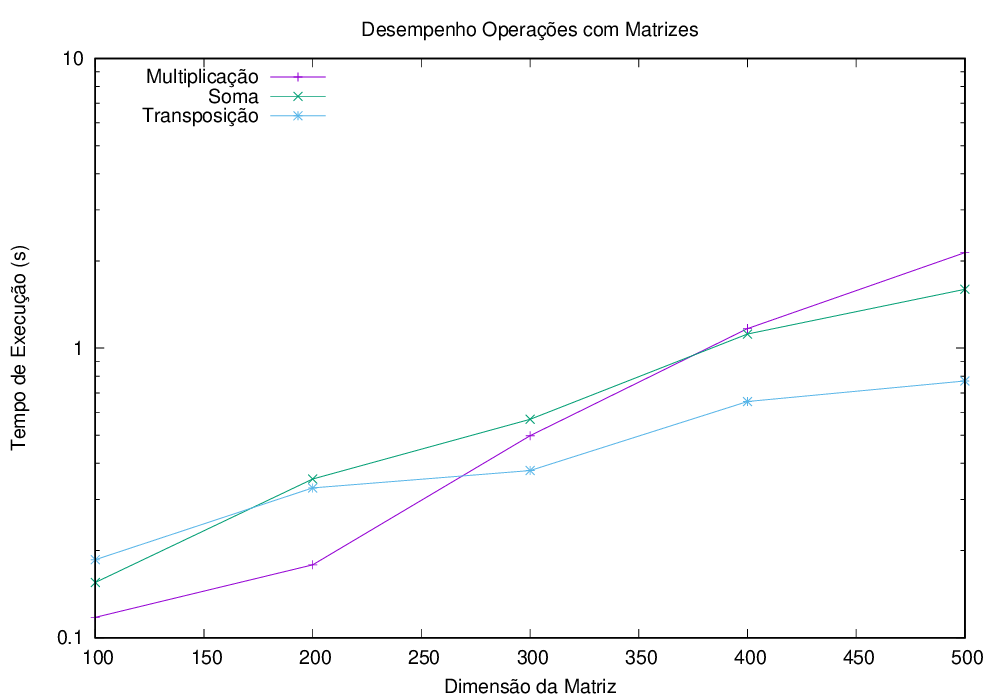
\includegraphics[width=10cm]{params-perf.png} 
    \centering
\end{figure}

Os arquivos de entrada foram matrizes \( n \times n \), em que todos os elementos eram ``5''. Essa escolha foi feita para minimizar possíveis variações de desempenho devido à presença de elementos menores ou maiores. Foram feitas 5 baterias de teste, a partir das quais foi feita uma média, que não considerou princípios estatísticos como o \textit{Desvio Padrão Relativo} e o \textit{Teste Q}.

Além disso, procurou-se minimizar o \textit{load} da máquina ao se realizar a análise, mantendo em execução apenas programas como o gerenciador de janelas (\textit{i3wm}) e um único terminal (\textit{kitty}) abertos (além de, claro, diversos processos importantes do sistema).

Apesar destas tentativas de redução de interferência, os dados estão relativamente inconsistentes. O esperado, pela análise de complexidade, é que a multiplicação seja muito mais custosa do que as outras operações; em segundo lugar a soma, que apesar de ter a mesma complexidade, faz mais operações e, em último a transposição.

Uma possível explicação para o comportamento observado é a verificação da validade dos arquivos: é uma tarefa relativamente custosa que escaneia cada arquivo mais de uma vez, e também analisa o arquivo resultante por segurança.

Para testar essa hipótese, foi feita uma análise semelhante à descrita no começo desta seção, mas sem o uso das funções de de arquivos comentadas. O resultado obtido está no gráfico a seguir: 

\begin{figure} [H]
    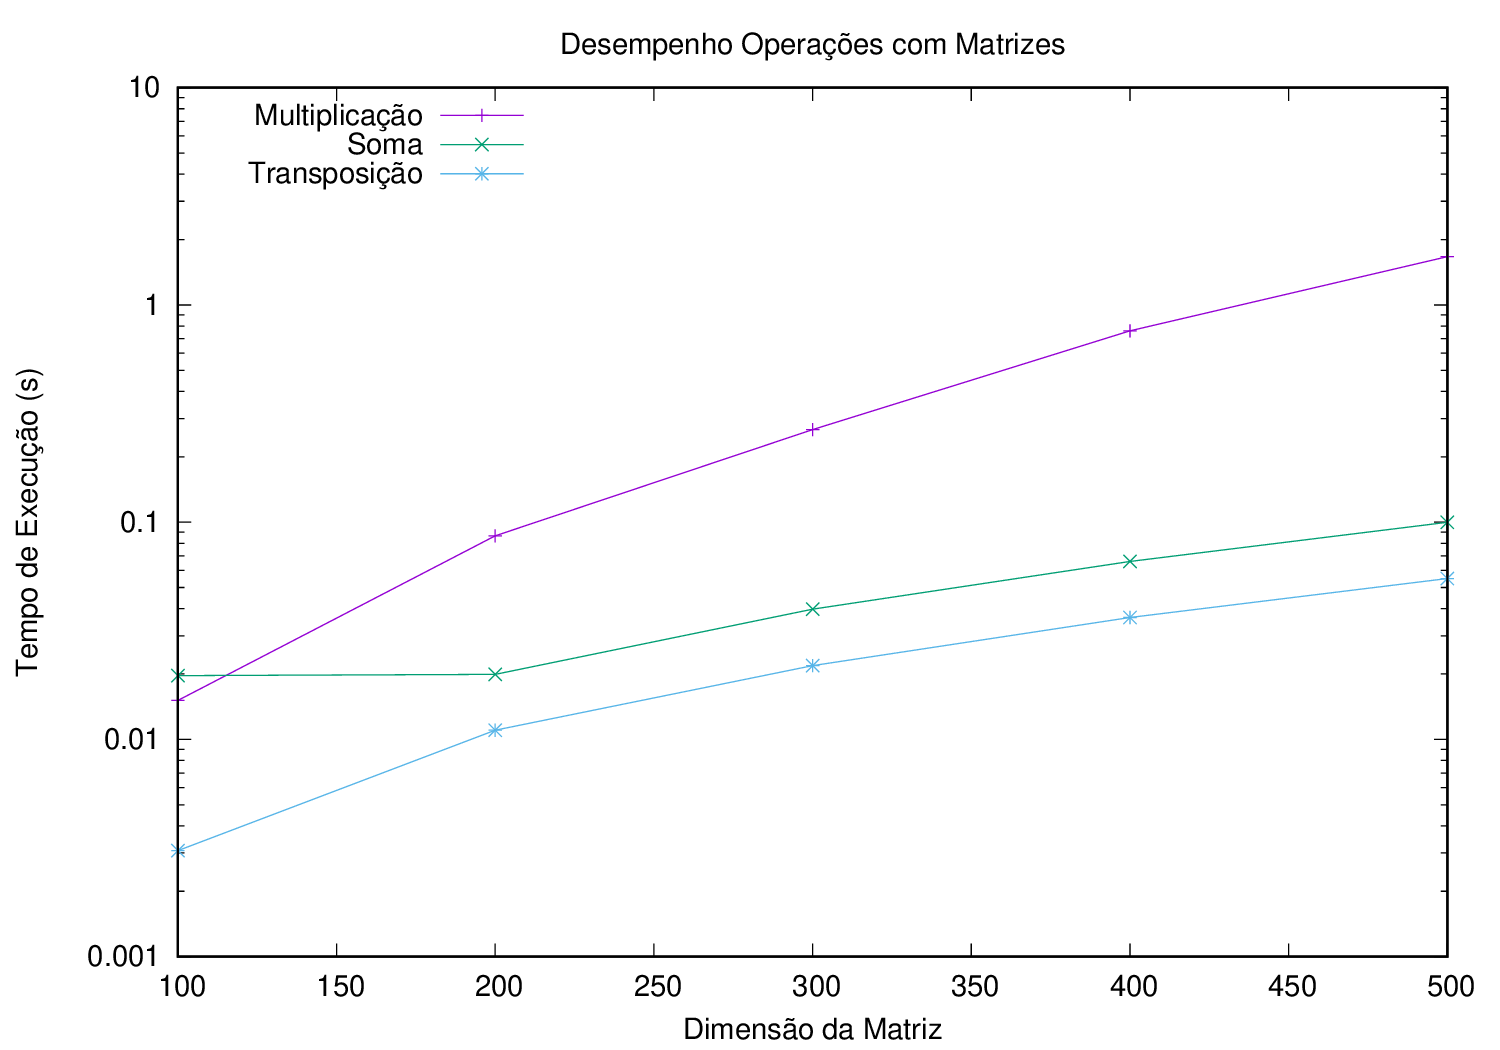
\includegraphics[width=10cm]{opt-params-perf.png} 
    \centering
\end{figure}

Estes dados são muito mais consistentes. Concluímos que a validação dos arquivos é o fator que ``segura'' a performance. De fato, para matrizes pequenas, essa diferença é tão relevante que coloca em cheque, por exemplo, a escolha do elemento ``5'' para ocupar toda a matriz. Se esse fosse um software de uso prático, poderia ficar à critério do usuário o grau de verificação dos arquivos -- afinal, foram escritos métodos que conferem questões específicas, como a primeira linha ou o número de linhas.

Outro aspecto analisado, mesmo que não tão meticulosamente, foi a influência dos valores dos elementos da matriz. Optou-se por utilizar a ``versão otimizada'' (que não confere a validade dos arquivos), por uma questão de praticidade. Foi usado como base os tempos de execução das operações para dimensão 300:

\begin{itemize}
    \item Multiplicação: 0.266993s
    \item Soma: 0.039785s
    \item Transposição: 0.0218501s
\end{itemize}

Para uma matriz cujos elementos variavam por coluna de 1 a 300 (mas as linhas eram idênticas), esse foi o resultado:

\begin{itemize}
    \item Multiplicação: 0.318661s
    \item Soma: 0.0441004s
    \item Transposição: 0.0246813s
\end{itemize}

Como esperado, a operação de transposição teve uma diferença marginal. A soma sofreu um aumento de aproximadamente 11\% e o produto de cerca de 19\%. Aqui, não há supresas: é intuitivo operações com números maiores demorarem mais.

\subsection{Eficiência de acesso à memória}

Nesta seção são apresentados alguns experimentos que avaliam a eficiência de acesso à memória do programa: padrão de acesso e a localidade de referência (distância de pilha). Para realizar essa tarefa, foi criada uma matriz \footnote{Esse tamanho é pequeno demais para visualizar uma propriedade da alocação dinâmica: nem sempre a memória é alocada em sequência. Podem haver ``saltos''.} \( 5 \times 5 \), com os elementos em sequência variando de 1 à 25, que foi usada como base para executar cada uma das operações do programa, com o registro de memória \textit{ativado}. Subsequentemente, foi utilizado o programa disponibilizado pelo prof. Wagner para gerar os mapas de acesso e histogramas.

É importante salientar que \textbf{essa análise foi feita estritamente a partir de manipulação de matrizes e exclui outras partes do programa}. Como foi visto na análise de performance, o efeito de, por exemplo, validação de arquivos pode ser não negligenciável.

O programa é dividido em 3 fases: inicialização da(s) matriz(es) de entrada (fase 0), realização da operação em questão (fase 1) e impressão (fase 2). No começo das fases 1 e 2, as matrizes utilizadas durante a fase são \textit{acessadas} com o método \code{acessaMatriz()}. Isso é importante pois é necessário ter um parâmetro para realizar a análise de pilha: sem um parâmetro não há comparação com relação ao seu \textit{último} uso, tornando-a sem sentido.

\subsubsection{Padrão de acesso}
O padrão de acesso é uma técnica que permite \textit{desenvolver uma noção} de como a memória está sendo utilizada, permitindo identificar possíveis gargalos. A seguir são discutidos os dados para cada uma das análises:

\paragraph{Transposição} Na transposição, só é lida uma matriz. Apesar disso, o programa foi implementado de tal modo que durante a transposição, outra matriz é criada. O padrão de acesso da matriz lida é:

\begin{figure} [H]
    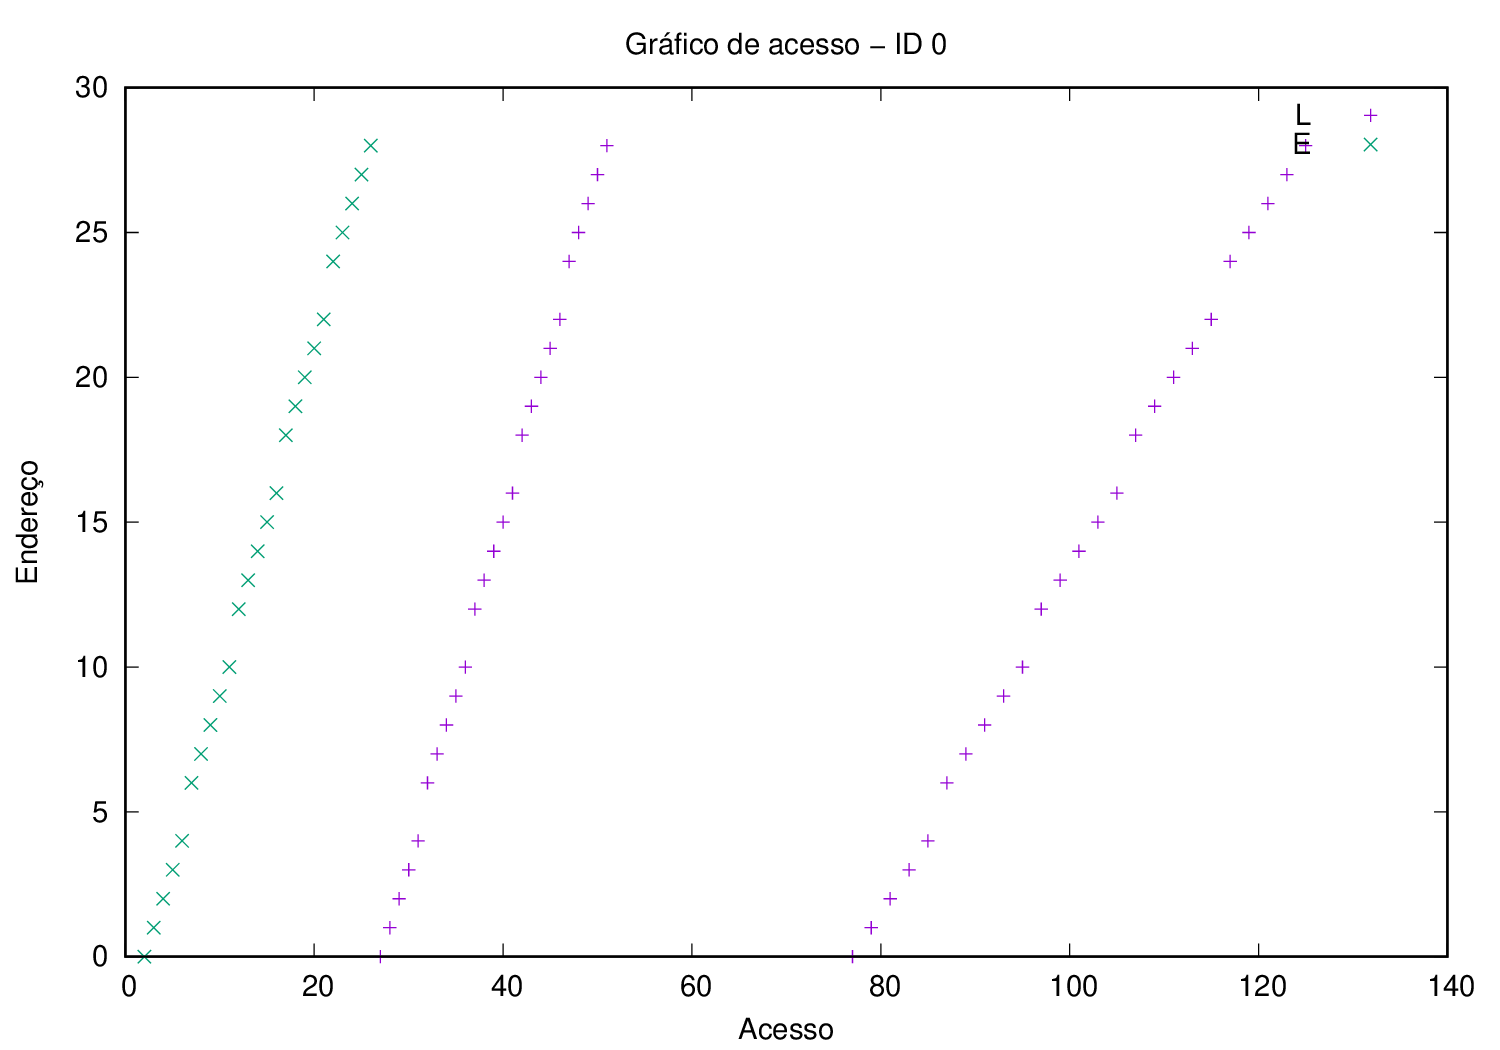
\includegraphics[width=10cm]{t-acesso-0.png} 
    \centering
\end{figure}

A escrita corresponde à associação a partir do arquivo de entrada. Em seguida, é usado o \code{acessaMatriz()} e o último bloco corresponde às chamadas sucessivas para transposição. O acesso da matriz resultante é:

\begin{figure} [H]
    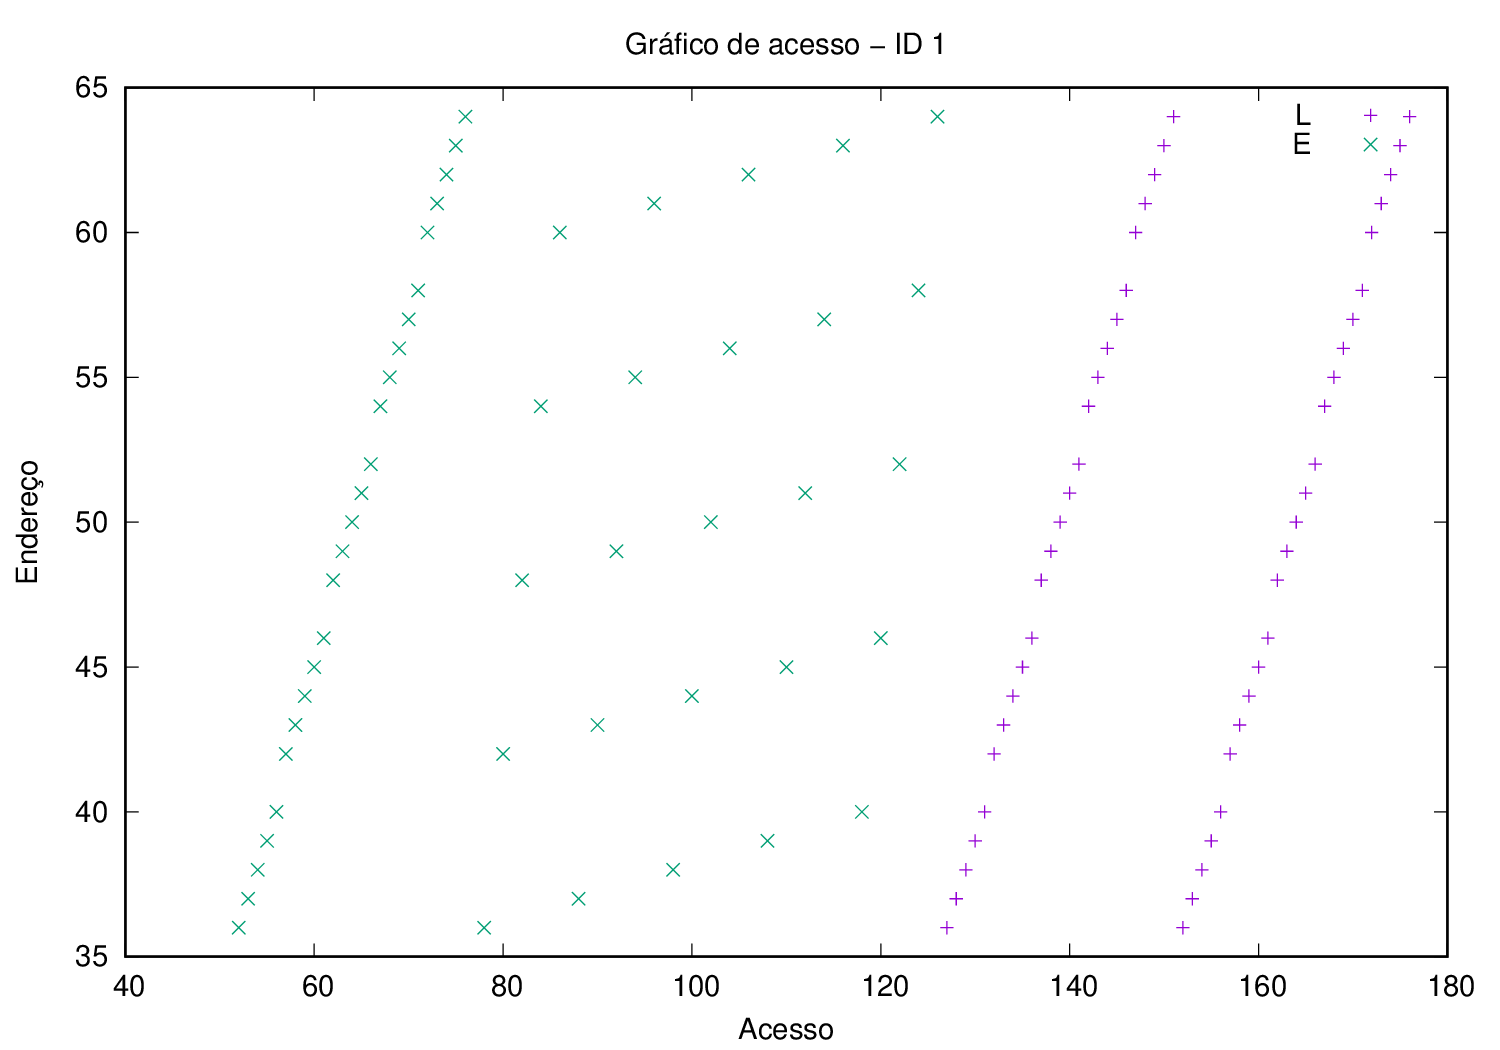
\includegraphics[width=10cm]{t-acesso-1.png} 
    \centering
\end{figure}

A primeira escrita se dá pelo uso do método \code{inicializaMatrizNula()}, a escrita seguinte é a transposição, que \textit{aparenta}\footnote{Na análise de pilha é mostrado que não é o caso.} não ser realizada de forma eficiente. A primeira leitura é o acesso e a outra a impressão.

\paragraph{Adição} Na adição são lidas duas matrizes, e há também a matriz resultante. O acesso das lidas é \textit{praticamente} idêntico à leitura da transposta e por isso foi omitido (os acessos são realizados na mesma ordem). Por outro lado, a matriz resultante apresenta comportamento diferente:

\begin{figure} [H]
    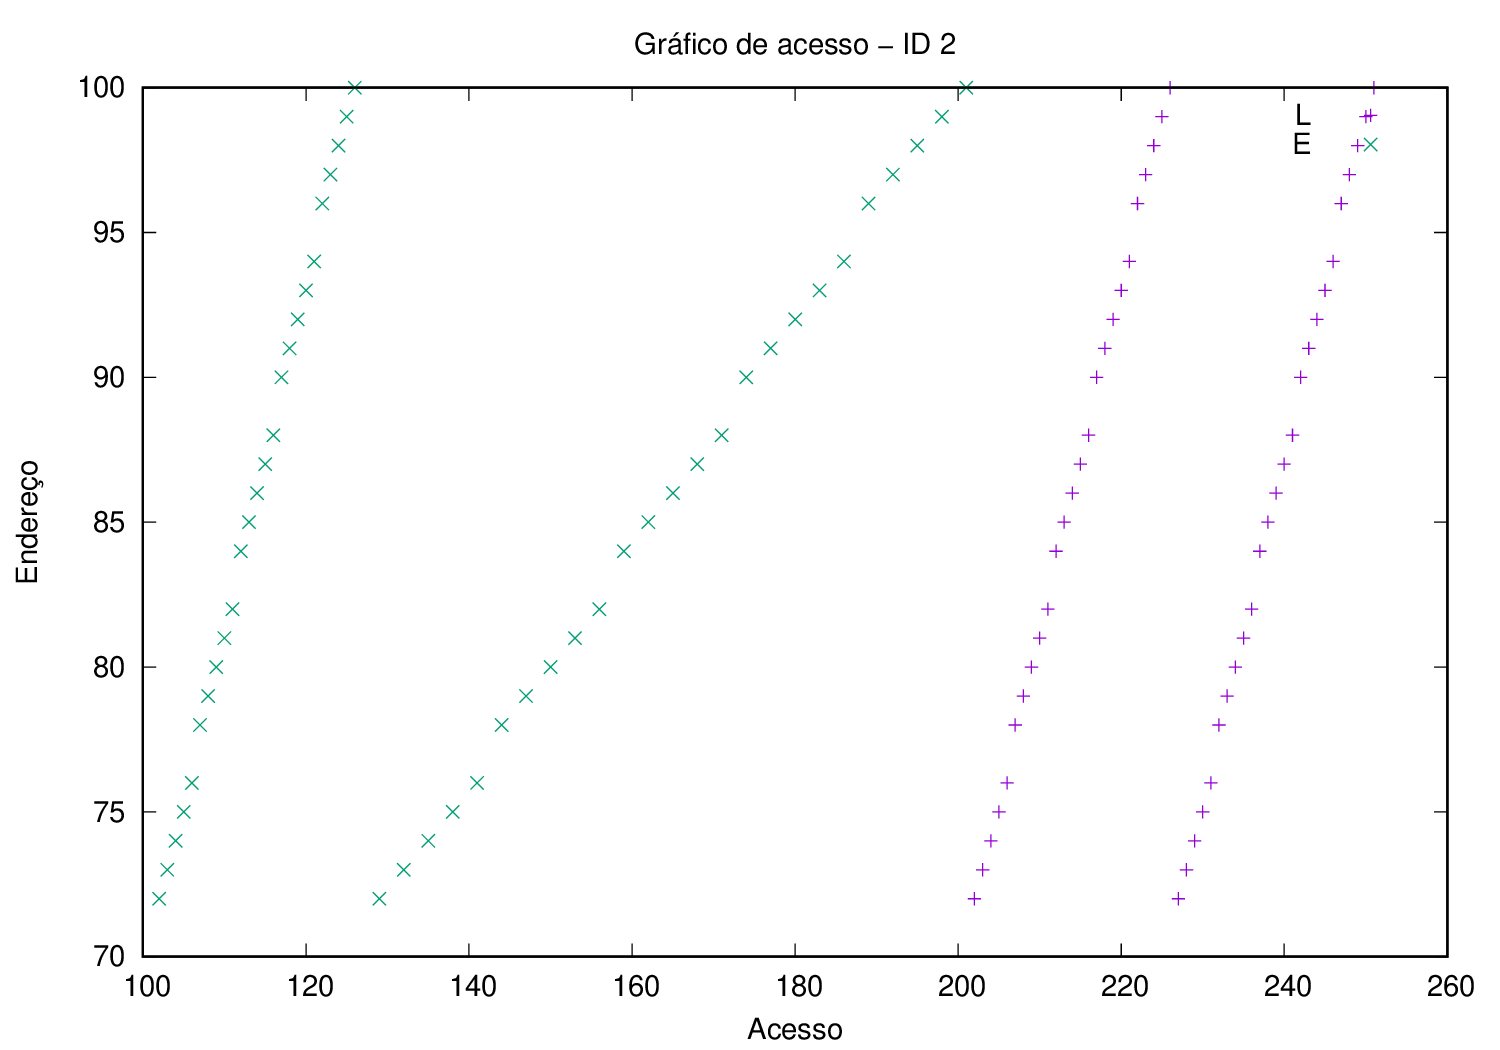
\includegraphics[width=10cm]{s-acesso-2.png} 
    \centering
\end{figure}

Aqui, a distinção em relação à transposição está na \textit{segunda escrita}, que é bem mais eficiente, por ser sequencial.

\paragraph{Multiplicação} a multiplicação funciona de forma fundamentalmente diferente das outras operações. A primeira matriz lida possui o seguinte perfil:

\begin{figure} [H]
    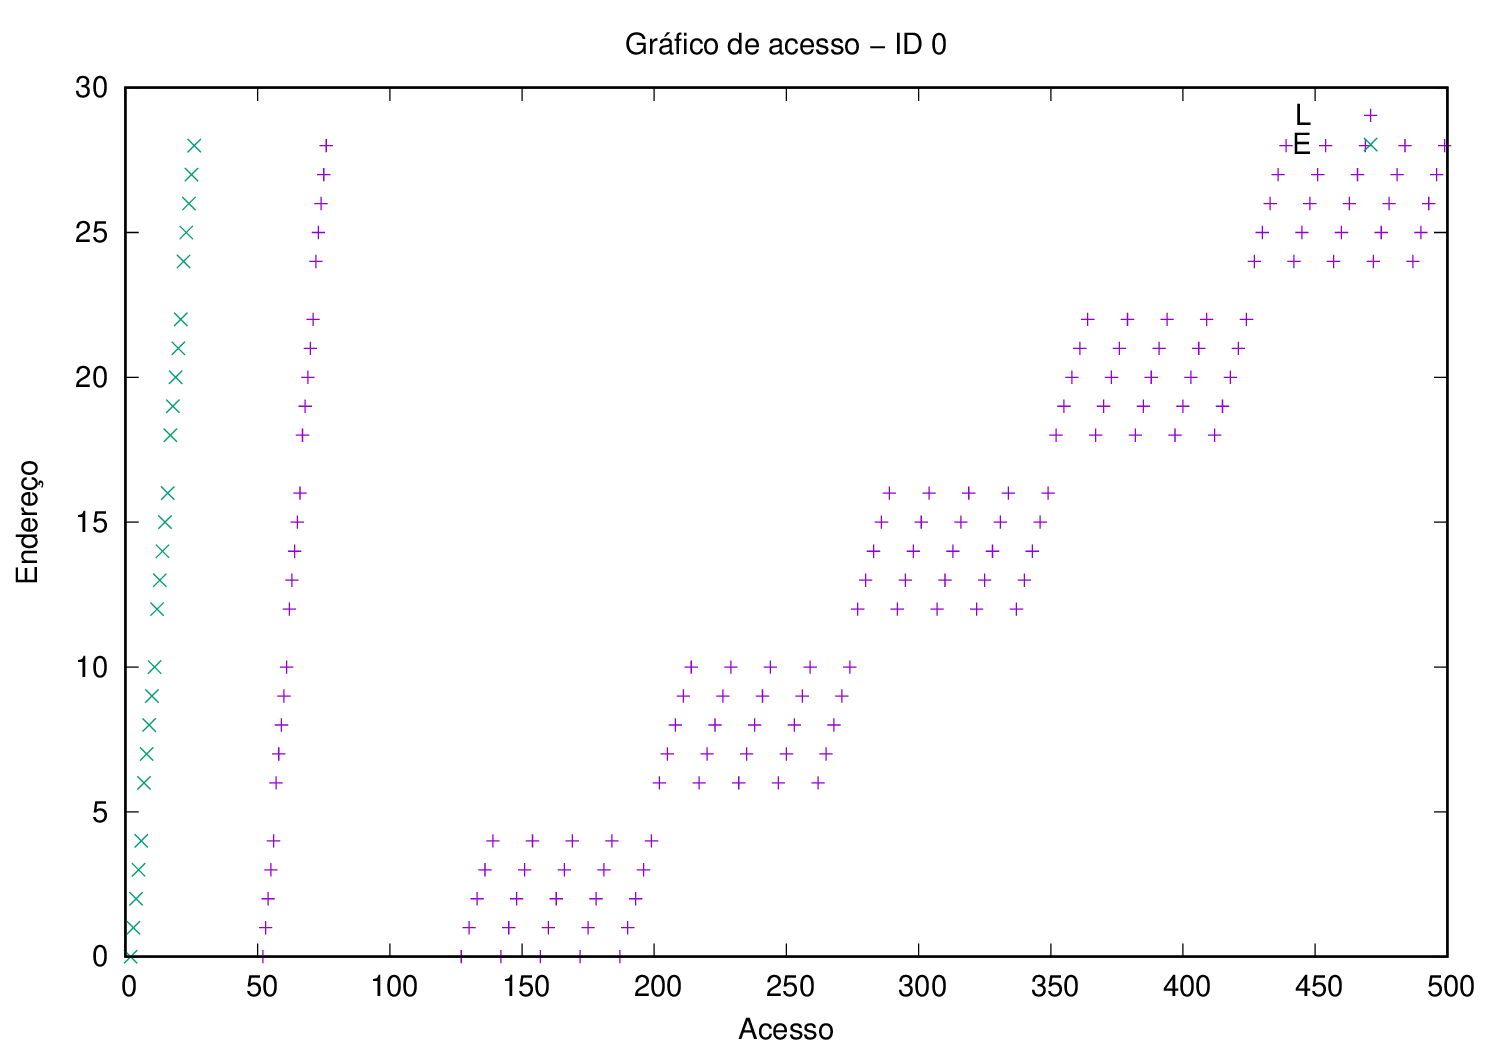
\includegraphics[width=10cm]{m-acesso-0.png} 
    \centering
\end{figure}

Notavelmente, a segunda leitura é sequencial por cada linha da matriz (por definição do produto de matrizes). Já no caso da outra matriz lida, tem-se:

\begin{figure} [H]
    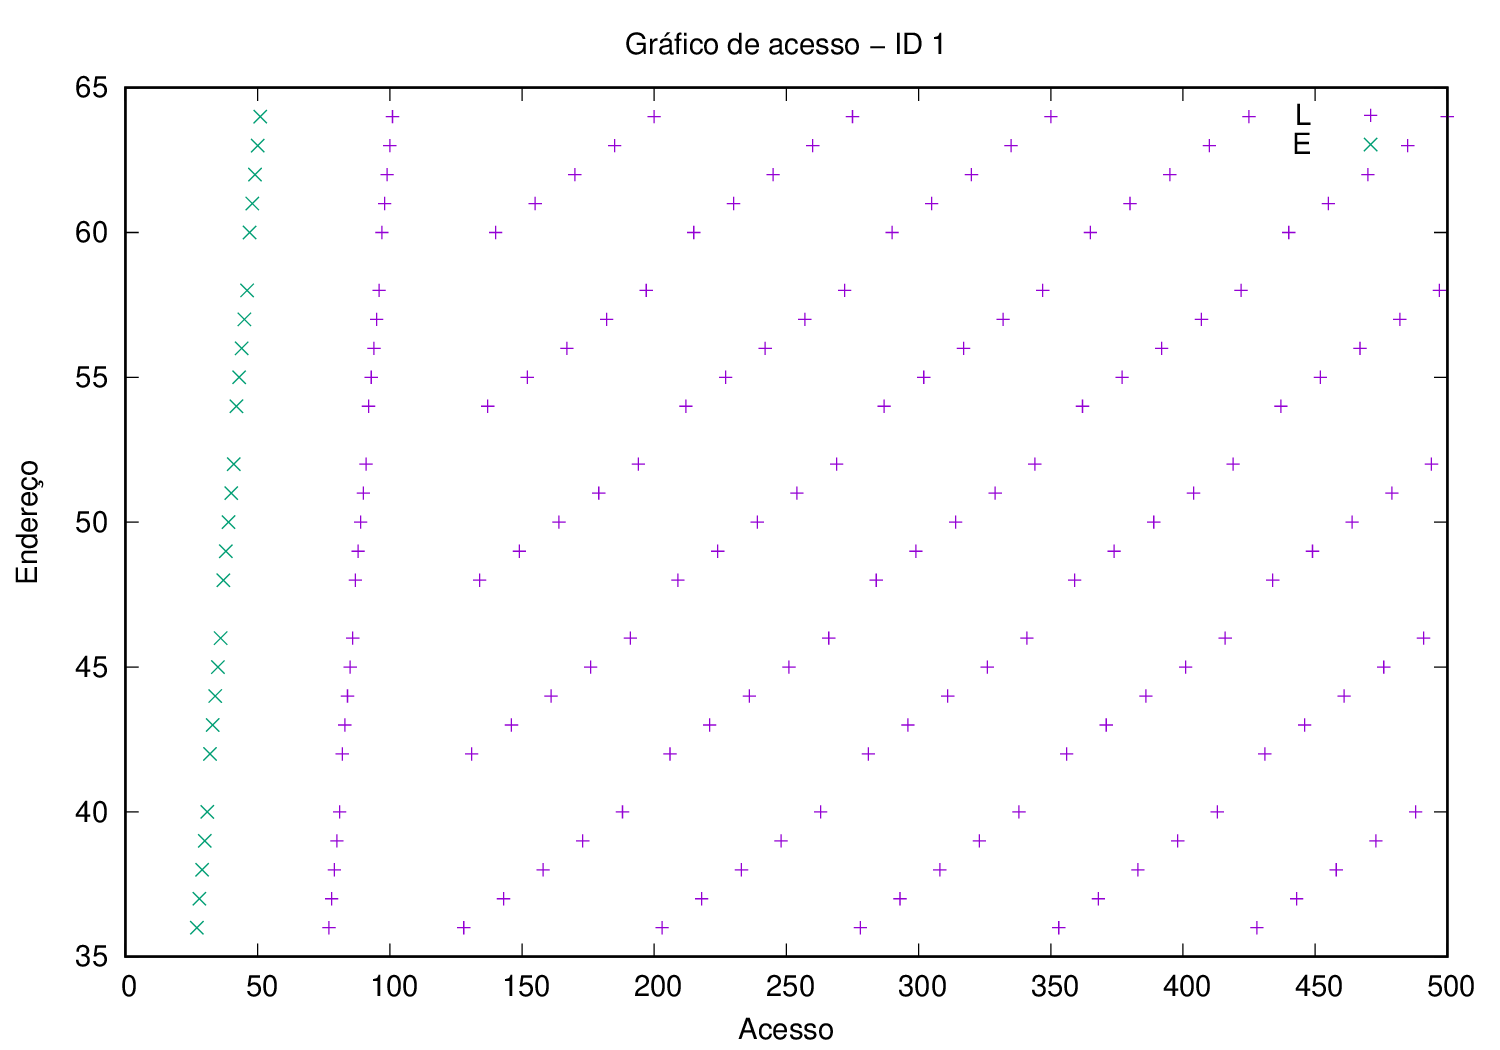
\includegraphics[width=10cm]{m-acesso-1.png} 
    \centering
\end{figure}

Aqui, a segunda leitura de se dá de forma muito ineficiente, com grandes ``saltos'': isso, porque na multiplicação, os elementos da segunda matriz são acessados por coluna, enquanto a memória está organizada por linhas. Para a última análise de acesso, tem-se o mapa de acesso da matriz resultante:

\begin{figure} [H]
    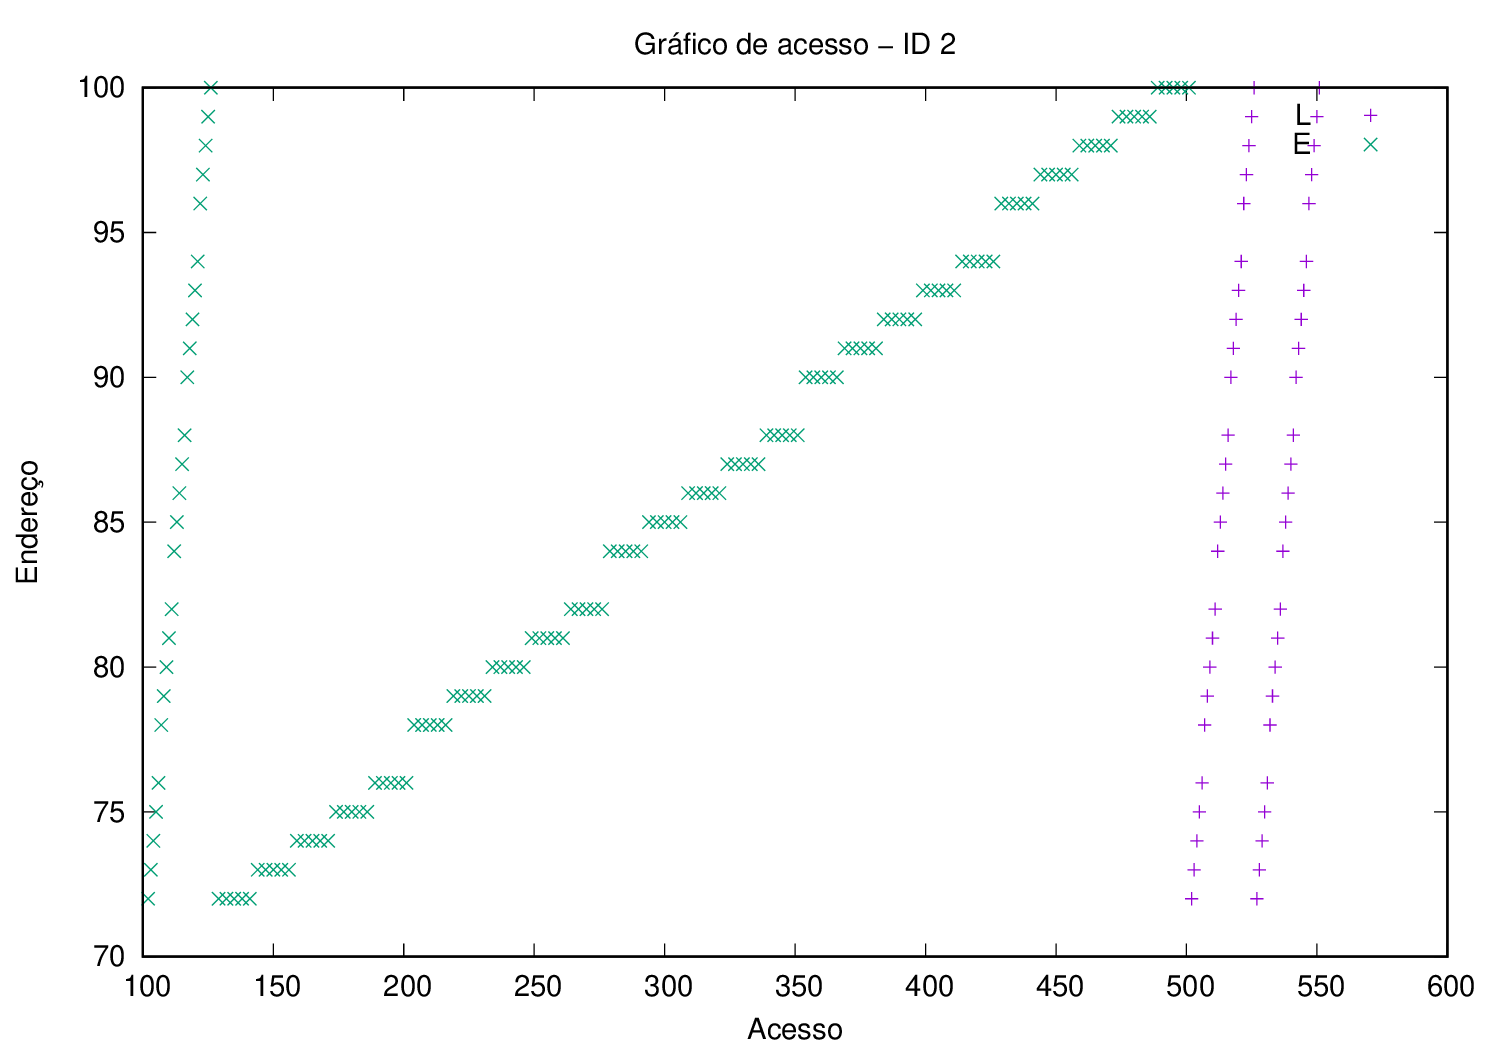
\includegraphics[width=10cm]{m-acesso-2.png} 
    \centering
\end{figure}

A primeira escrita é uma inicialização nula, a segunda é sequencial, mas é tomada a soma \( k \) vezes (em que \( k \) é o número de colunas da 1ª matriz).

\subsubsection{Localidade de Referência}

Para medir a localidade de referência, foi feita uma análise da distância de pilha (DP) em cada fase do programa, que será exposta a seguir. Alguns casos mais simples serão apenas comentados, evitando assim a inclusão de figuras desnecessariamente. Em especial, a fase 0 nunca é interessante: não há referência e sempre se assume uma distância de 0. Além disso, a fase 2 também nunca é interessante: ocorre apenas o acesso (distância 0) e a impressão sequencial (distância 25\footnote{Generalizando, \( nm \). Todo número apresentado explicitamente nesta seção é facilmente generalizável (desconsiderando questões de ``salto'' na alocação dinâmica).}), obtendo uma DP de 625.

\paragraph{Transposição} Na fase 1, é apresentado comportamento trivial para a matriz de entrada, que é idêntico ao da fase 2. No entanto, a matriz resultante apresenta peculiaridades:

\begin{figure} [H]
    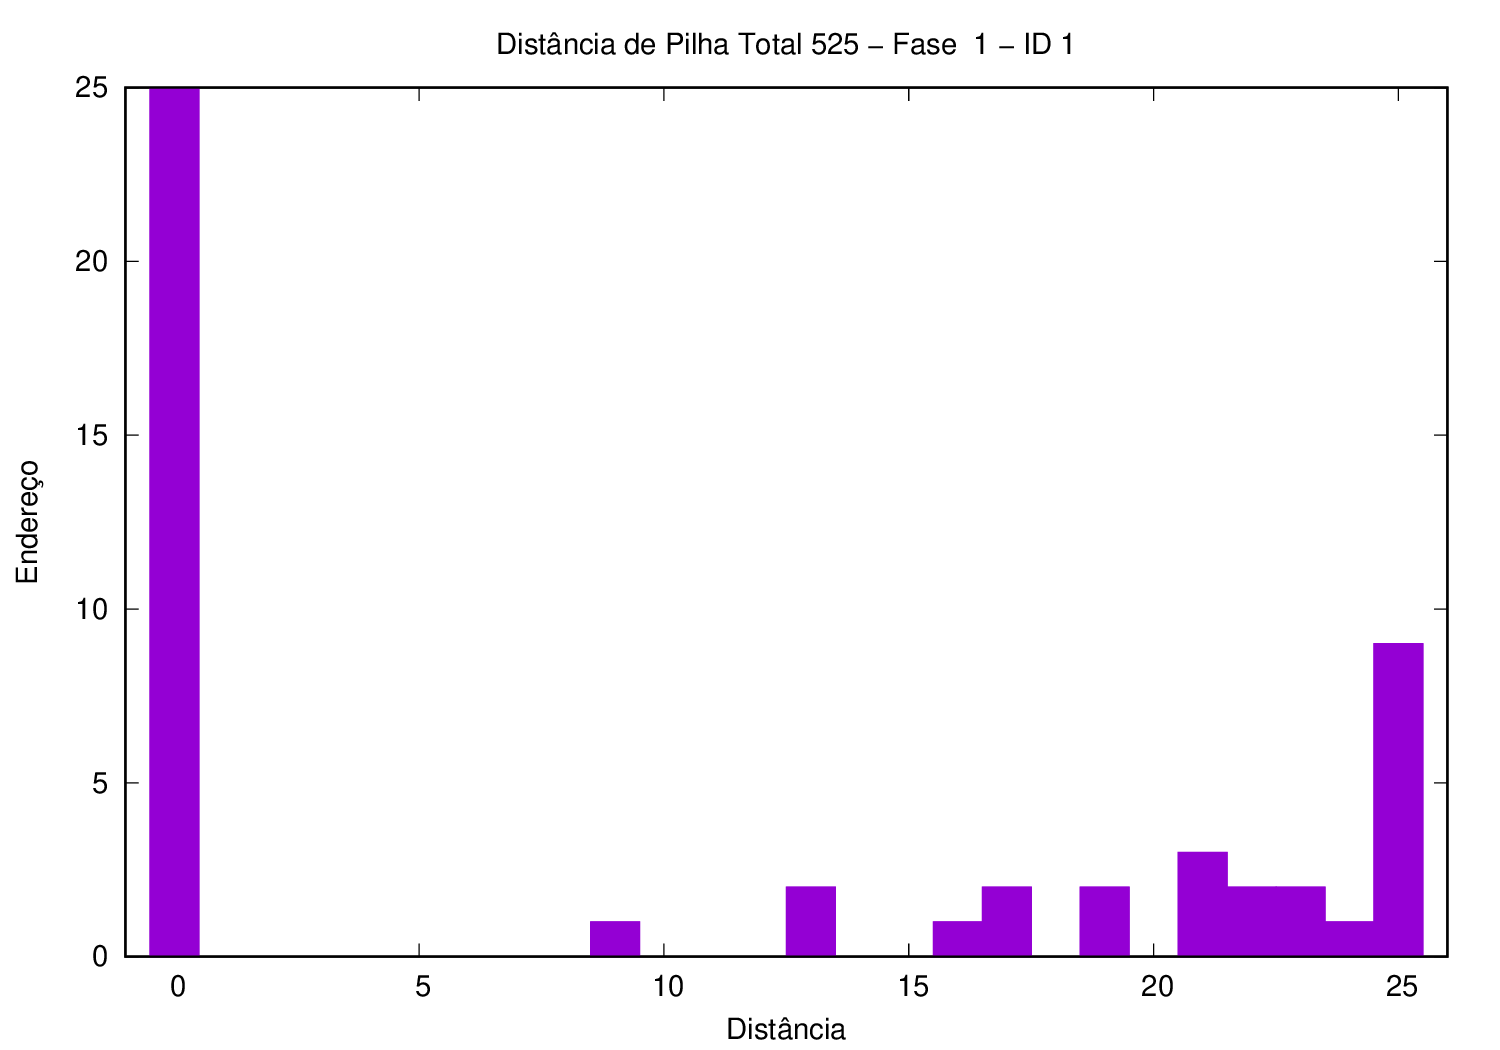
\includegraphics[width=10cm]{t-hist-1-1.png} 
    \centering
\end{figure}

Os acessos zerados correspondem a uma inicialização nula. Os outros representam a não linearidade observada no mapa de acesso da escrita da tranposição: é comum os elementos serem acessados a uma distância de 25, mas a maioria dos elementos é ``adiantada'' algumas posições (pela operação se basear em colunas e o armazenamento em linhas). Considere, por exemplo, o elemento na posição [5][1]: um dos últimos a serem acessados pelo \code{acesaMatriz()}, mas com o deslocamento ``vertical'' da transposição, ele rapidamente é acessado de novo (distância 9).

\paragraph{Soma} É uma operação (não) surpreentemente simples: em todas as fases o acesso às matrizes só é realizado o acesso sequencial (como discutido anteriormente), mantendo a DP de 625 para cada etapa.

\paragraph{Multiplicação} Na fase 1, cada matriz tem um acesso distinto. A começar pela primeira matriz de entrada:

\begin{figure} [H]
    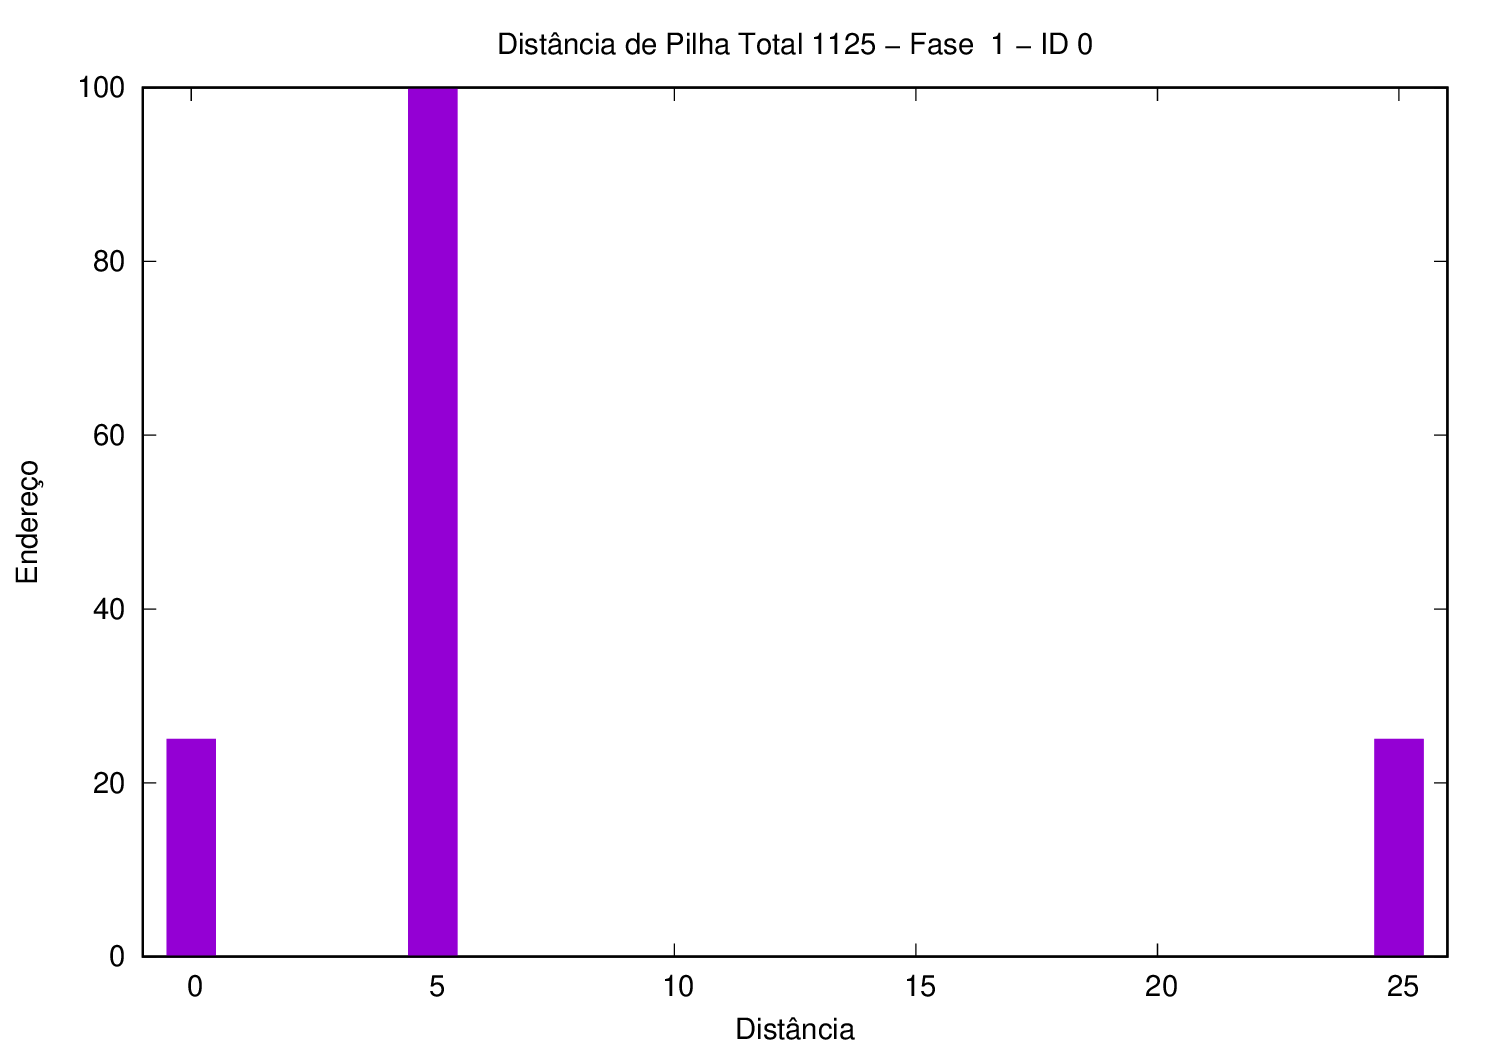
\includegraphics[width=10cm]{m-hist-1-0.png} 
    \centering
\end{figure}

Os acessos zerados correspondem ao método \code{acessaMatriz()}. A grande quantidade de distâncias 5 se dá pelo caminhamento do produto: para cada coluna da 2ª matriz, acessamos a mesma linha. Como as matrizes em questão são \( 5 \times 5 \), e o produto é implementado de tal modo que a matriz resultante é calculada linha a linha, a cada mudança de coluna os elementos da linha da 1ª matriz são acessados. Os acessos com uma DP de 25 são os primeiros acessos a uma dada linha. A segunda matriz de entrada é mais ``caótica'':

\begin{figure} [H]
    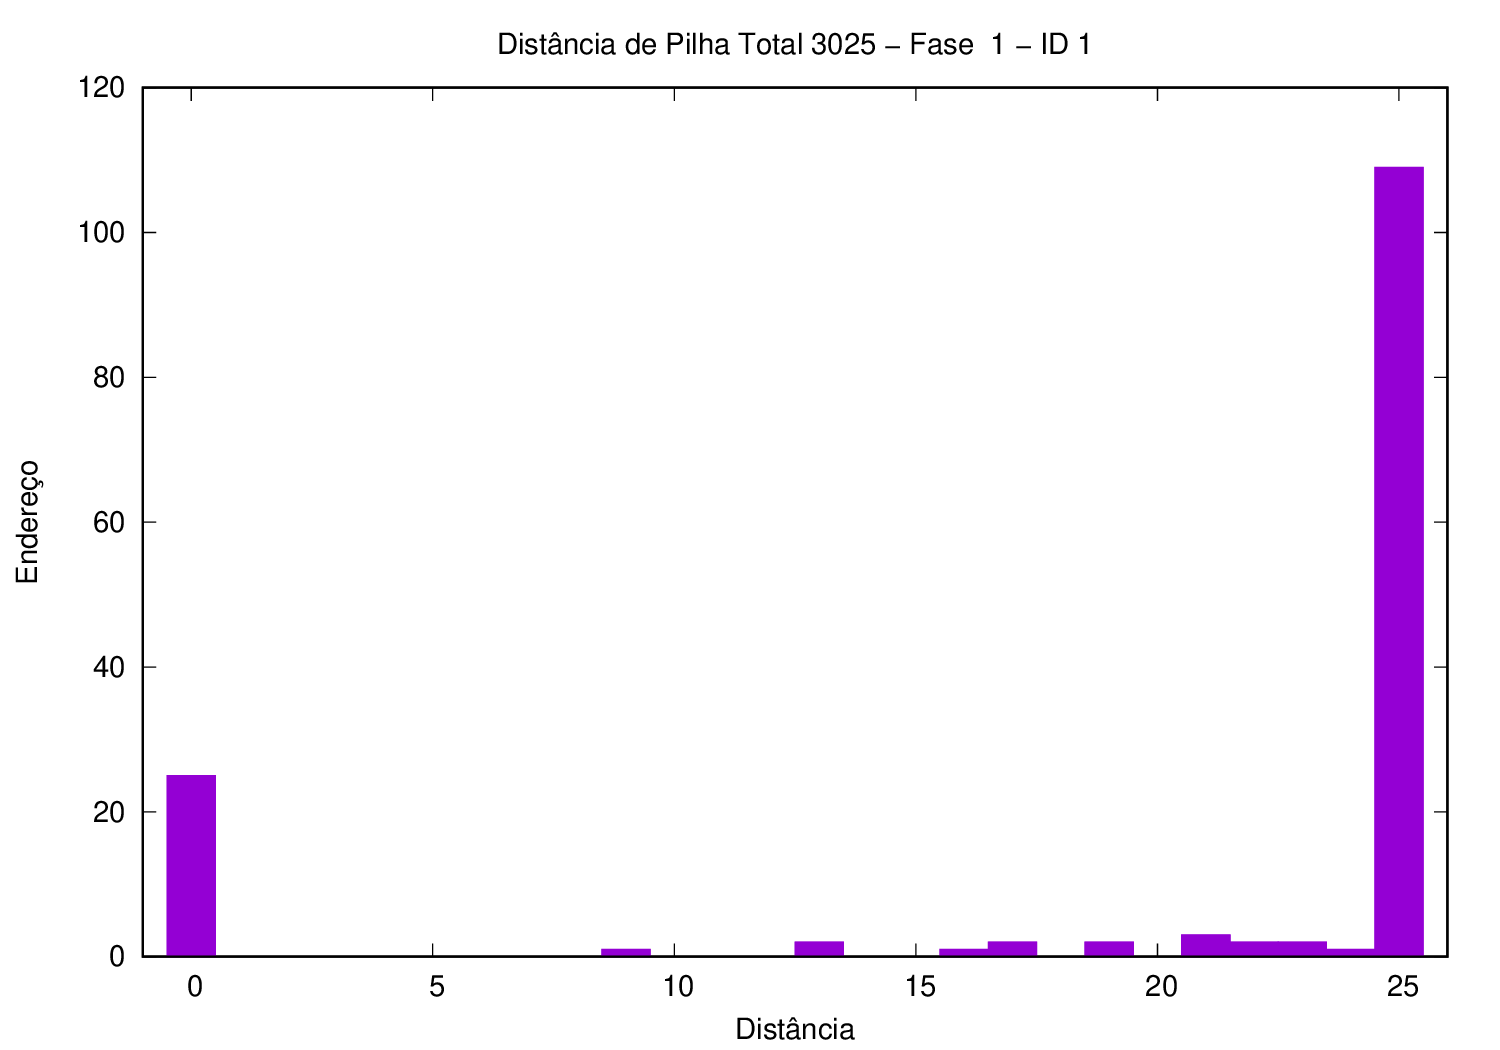
\includegraphics[width=10cm]{m-hist-1-1.png} 
    \centering
\end{figure}

Mais uma vez temos o \code{acessaMatriz()}. Mas os outros 125 acessos se dão de maneira muito menos intuitiva. A vasta maioria destes possui DP de 25, mas como no caso da transposição, o acesso mais ``vertical'' acaba adiantando alguns quando a primeira linha da matriz resultante está sendo calculada. Depois disso, o acesso é repetido para se obter as outras linhas (o que explica o alto número de distâncias 25). Esse é um ótimo estudo de caso que suporta a ineficiência da implementação para realizar essa operação.

Finalmente, temos a última análise de pilha desta documentação: a matriz resultante da multiplicação.

\begin{figure} [H]
    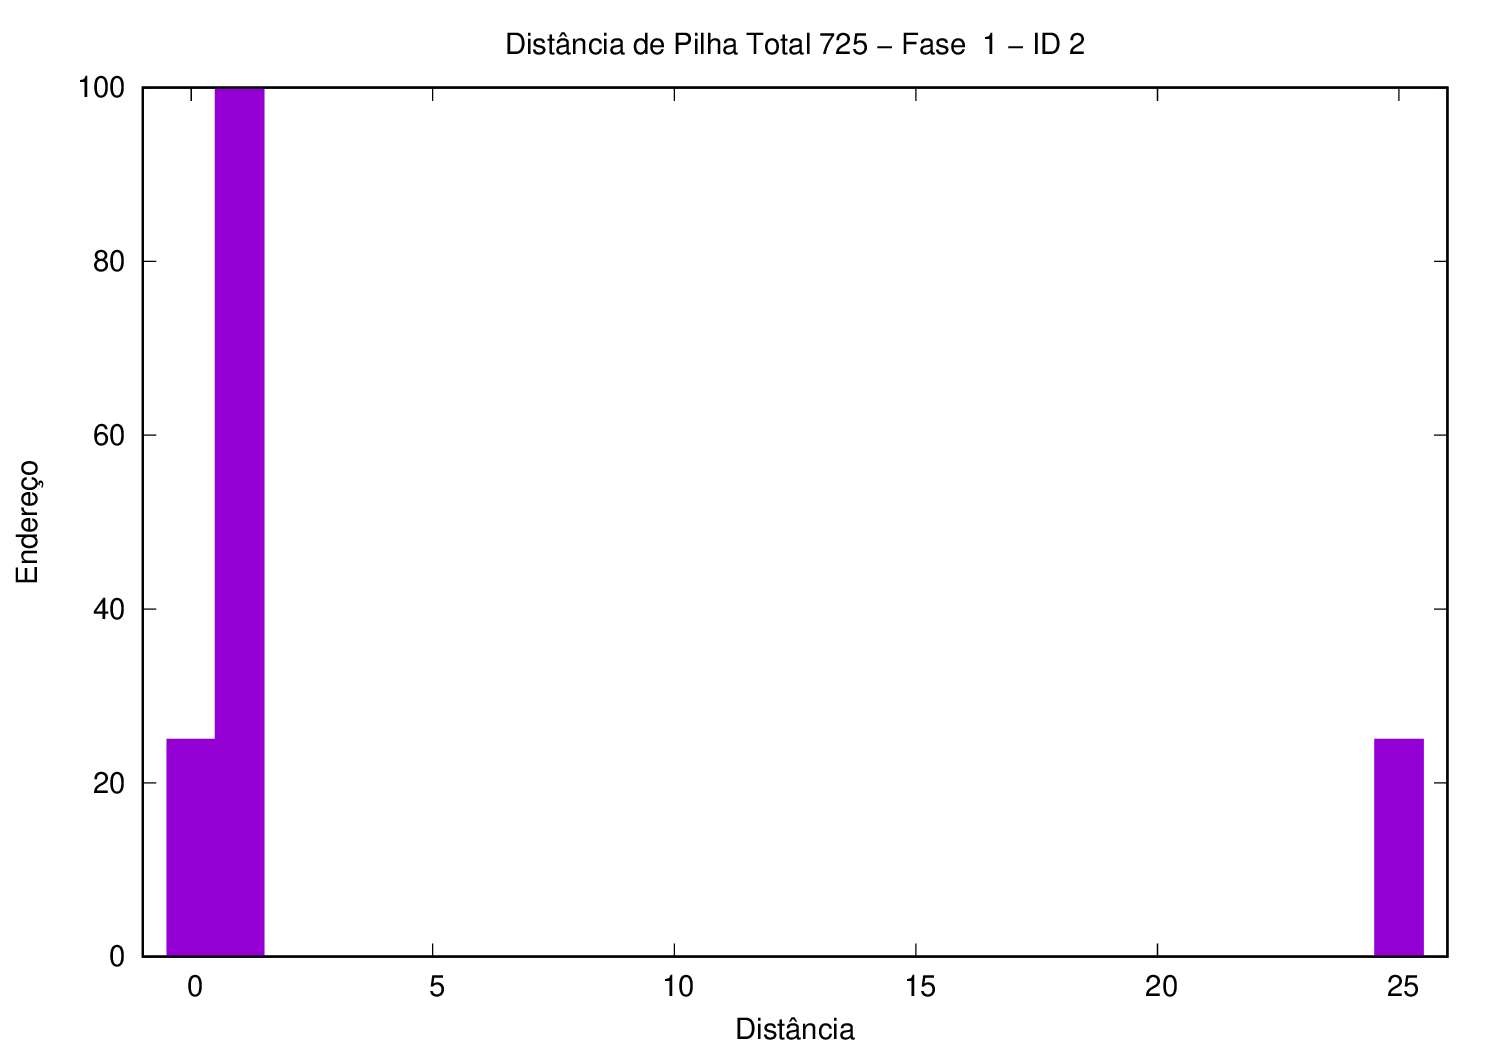
\includegraphics[width=10cm]{m-hist-1-2.png} 
    \centering
\end{figure}

Aqui há os acessos nulos do \code{inicializaMatrizNula()} e, cada elemento, uma vez acessado, ainda recebe mais 4 somas (o que explica as 100 distâncias 1). Os 25 acessos de 25 correspondem ao descolamento sequencial pela matriz. Um detalhe interessante aqui é que, as operações em sequência para um mesmo elemento \textit{não interferem} no fato de a distância de pilha ser 25, pois cada vez que um endereço é acessado, ele é colocado no topo da pilha (ou seja, não é contado, como seria o caso de um endereço distinto).

Assim, concluímos as análises de eficência de acesso à memória.

\section{Conclusões}

Neste trabalho foi implementado um programa que realiza algumas operações sobre matrizes alocadas dinamicamente, que são lidas de arquivos a partir de parâmetros da linha de comando. O que parece uma tarefa relativamente simples, ainda mais com um TP de exemplo para servir de guia, mas acabou se provando uma tarefa não-trivial que exigiu horas e horas de dedicação.

\subsection{Aprendizado Pessoal}

\textit{Esta seção está escrita em 1ª pessoa intencionalmente.}

Em questões de implementação e estruturas de dados, não houve muito o que aprender: matrizes são conhecidas, e ter uma base para o trabalho simplificou bastante o processo de escrever o código em si. Foi interessante portar o código para C++, e também a parte de tratar os arquivos.

Uma área de aprendizado bastante desenvolvida por mim nesse trabalho engloba uma série de tangências: precisei entender e configurar os testes usando o GoogleTest e escrevi essa documentação usando \LaTeX, que foi uma tarefa surpreendemente complicada em alguns pontos (apesar de já ter certa familiaridade com a ferramenta). 

\textit{Fazer o título} o mais semelhante que pude ao especificado, por exemplo, exigiu certa engenhosidade. Tive uns problemas de \textit{encoding} e descobri como formatar melhor para português: normalmente, ao copiar um trecho do arquivo final, os acentos e afins ficam todos quebrados. Mas tem um jeito de resolver isso (que traz outros benefícios também). Você, corretor, pode testar que os acentos e tis funcionam copiando algum trecho. Outra questão sobre o \LaTeX\  foi incluir as imagens geradas pelo \textit{gnuplot}. Isso exigiu certo \textit{troubleshooting} que no final acabei nem conseguindo resolver e optei por converter fora do documento, usando o comando \textit{convert} do software \textit{ImageMagick} (e posteriormente o comando \textit{mogrify}).

O fato de eu ter mencionado dificuldades mais tangentes provavelmente se deve a elas serem mais recentes. Mas não foi só isso: fazer as análises de complexidade e de desempenho também não foi uma tarefa simples. Acho que as orientações, em particular com as análises de \textit{eficiência de acesso à memória} no que diz respeito à criação dos gráficos ficou meio ``solta'' (mesmo eu tendo conseguido fazer, precisei quebrar a cabeça). De forma geral, fiquei incomodado com a distruibuição de pontos: as análises de complexidade valem \( \frac{1}{4} \) da nota, e temo perder alguns pontos apesar de ter me esforçado muito em outras etapas da execução do trabalho. Estou relativamente confiante nas minhas análises de tempo, mas nas de espaço já tenho incertezas.

Também não sei se aprofundei o suficiente nas análises de eficiência de memória ou se deveria ter dado uma ênfase maior nas divergências com relação à alocação estática (como comentado antes, imagino que 5 é um tamanho pequeno para ver isso). Mas no que testei com tamanhos maiores, a visualização de alguns gráficos não fica tão boa (talvez seria questão de encontrar um meio termo).

Apesar de não saber como vou ser avaliado, modestia à parte, meu aprendizado e esforço produziram um ótimo trabalho. Gostei bastante do resultado final, e não vejo como poderia ter feito um trabalho melhor.

\section{Bibliografia}
Apesar de não ter citado nada diretamente, o TP de exemplo e as aulas foi de grande ajuda. Assim como as aulas específicas sobre isso, do Professor Wagner Meira Júnior. Aqui está formatada em ABNT apenas uma das aulas, embora todas tenham contribuído.

JÚNIOR, Wagner Meira. \textbf{Tipos Abstratos de Dados Matriz}. [S. l.], 3 nov. 2021. Disponível em: shorturl.at/qrQ19. Acesso em: 4 nov. 2021.

JÚNIOR, Wagner Meira. \textbf{TP 0 com matrizes estáticas.} [S. l.], 21 out. 2021. Disponível em:shorturl.at/pEHR5. Acesso em: 31 out. 2021.

\newpage

\section*{Instruções}

\subsection*{Compilação}

Você pode compilar o programa da seguinte maneira:

\begin{enumerate}
    \item Abra um terminal;
    \item Utilize o comando \code{cd} para mudar de diretório para a localização da raiz do projeto;
    \item Utilize o comando \code{make}. 
\end{enumerate}

Pronto! O programa principal foi compilado. \textit{Opcionalmente,} você também pode usar o comando \code{make test} para compilar e rodar um arquivo com (alguns) testes. Mas \textbf{lembre-se:} é \textbf{preciso} ter o GoogleTest instalado \textbf{globalmente} em sua máquina!

\subsection*{Execução}

Você pode rodar o programa da seguinte maneira:

\begin{enumerate}
    \item Abra um terminal;
    \item Utilize o comando \code{cd} para mudar de diretório para a localização da raiz do projeto;
    \item Utilize o comando \code{./bin/matop [args]}, em que \code{args} são os argumentos que você deseja usar. 
\end{enumerate}

Atente-se pois nem toda combinação de argumentos é válida, e os arquivos devem estar \textit{exatamente} como descrito na seção de robustez.

\end{document}
